\subsection{Parameter Estimation}\label{sectionEstimation}

In order to reach successful performance in real robot table tennis, accurate ball prediction models are needed. For this purpose, we collect data from a human table tennis demonstration recording and estimate the parameters of the ball models. In these sessions, we record the ball position observations from the cameras as well as the robot joint angles. A ball-launcher is used to launch balls with high topspin. The noisy dataset of human table tennis demonstrations 
%
\begin{align}
\dataset = \{\vec{t}_i, \ball_i, \joint_i\}_{i=1}^{N} \label{demonstrations},
\end{align}
%
\noindent consists of $N = 90$ trials. Each trial $i$ contains $M_i$ ball position and $K_i$ joint position recordings sorted by time, i.e.,
%
\begin{align}
\ball_i &= \{\ball_{ij}\}_{j=1}^{M_i}, \joint_i = \{\joint_{ij}\}_{j=1}^{K_i},
\end{align}
%
\noindent sorted by $\vec{t}_i = \{t_{ij}\}_{j=1}^{K_i}$. Typically $K_i > M_i$, e.g., for the Barrett WAM, we record the robot joint values with a frequency of $500$ Hz, whereas our vision system outputs ball observations at around $60$ Hz.

Whenever the future path of the ball is predicted with the ball models, the accuracy of the predictions using the rebound model~\eqref{reboundModel} and the racket contact model~\eqref{contactModel} clearly depend on that of the flight model~\eqref{flightModel}. Hence we first start by estimating the parameters of the flight model using nonlinear least squares (NLS). We collect the time stamps and the ball positions detected by the vision system before rebound. The rebound index for each trial $i$ is estimated as
%
\begin{align}
j_b(i) &= \arg\min_{j} b_{z_{ij}}, \\
\textrm{s.t. \ }
& -\tfrac{w_{T}}{2} \leq b_{x_{ij}} \leq \tfrac{w_{T}}{2}, \\
& \ y_{\mathrm{edge}} - l_{T} \leq b_{y_{ij}} \leq y_{\mathrm{edge}}.
\label{bounceTimeEst}
\end{align}
%
We then use all of the observations until rebound, $\{(t_{ij},\ball_{ij})_{j=1}^{j_b(i)}\}$, to estimate the parameters $\gravity$, $\drag$ and $\lift$. This procedure requires to estimate as well the trial specific topspin parameter, i.e., $\spin = (0,0,\omega_z)^{\mathrm{T}}$ for some topspin value $w_z$, separately for each trial $i = 1 \ldots, N$. % i.e., ball measurements before $b_z < z_{\mathrm{TABLE}}$. 

We use the flight model with the estimated parameters to smoothen the ball path before rebound and after rebound. Using an Extended Kalman Smoother~\citep{Sorenson85}, the ball velocities are calculated before and after rebound, $\dot{\ball}_{\mathrm{in}}, \dot{\ball}_{\mathrm{out}}$ respectively. NLS is again used to estimate the rebound parameters $\coeffFrictionTable$ and $\coeffRestitutionTable$. See Figure~\ref{trainBounce} for an illustration. %The estimated rebound parameters can compensate for the effects of spin, assuming that the spin is approximately the same throughout the demonstrations.

\begin{figure}[t!]
	\centering
	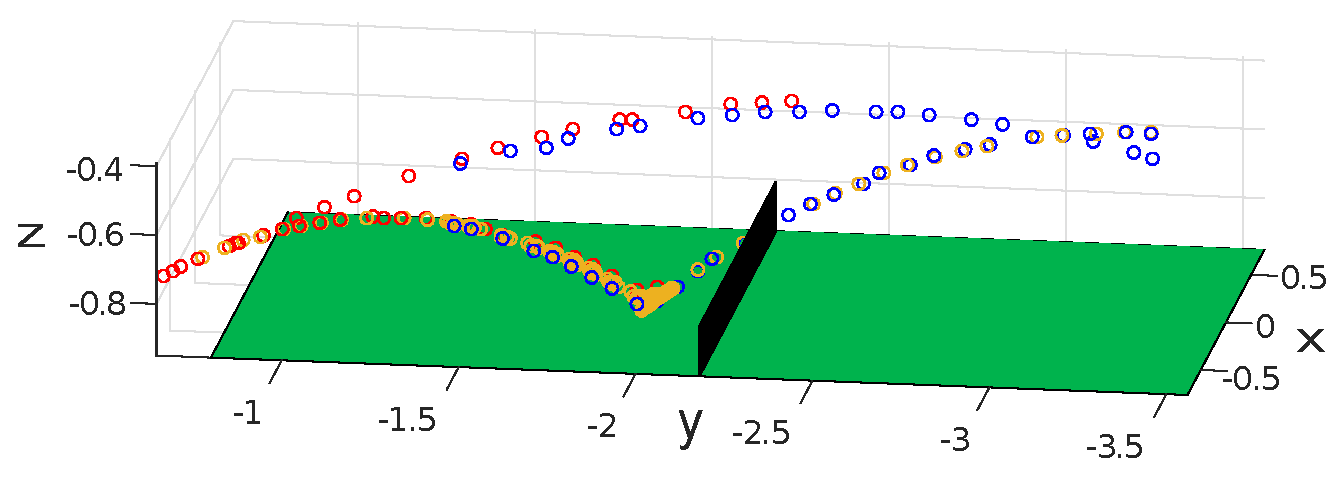
\includegraphics[scale=0.35]{trainBounce.eps}			
	\caption{Using Extended Kalman Smoothing (EKS) to estimate the parameters of the rebound model from actual noisy ball data during a demonstration recording. Ball observations are acquired from two different sets of cameras on opposite sides of the table, shown as red and blue circles respectively. They are then smoothened with the EKS, shown in yellow, to obtain velocity estimates before rebound and just after rebound. Nonlinear least squares is then used to estimate the rebound model parameters $\coeffFrictionTable$ and $\coeffRestitutionTable$.} 
	\label{trainBounce}
\end{figure}

%\begin{figure}
%	\centering
%	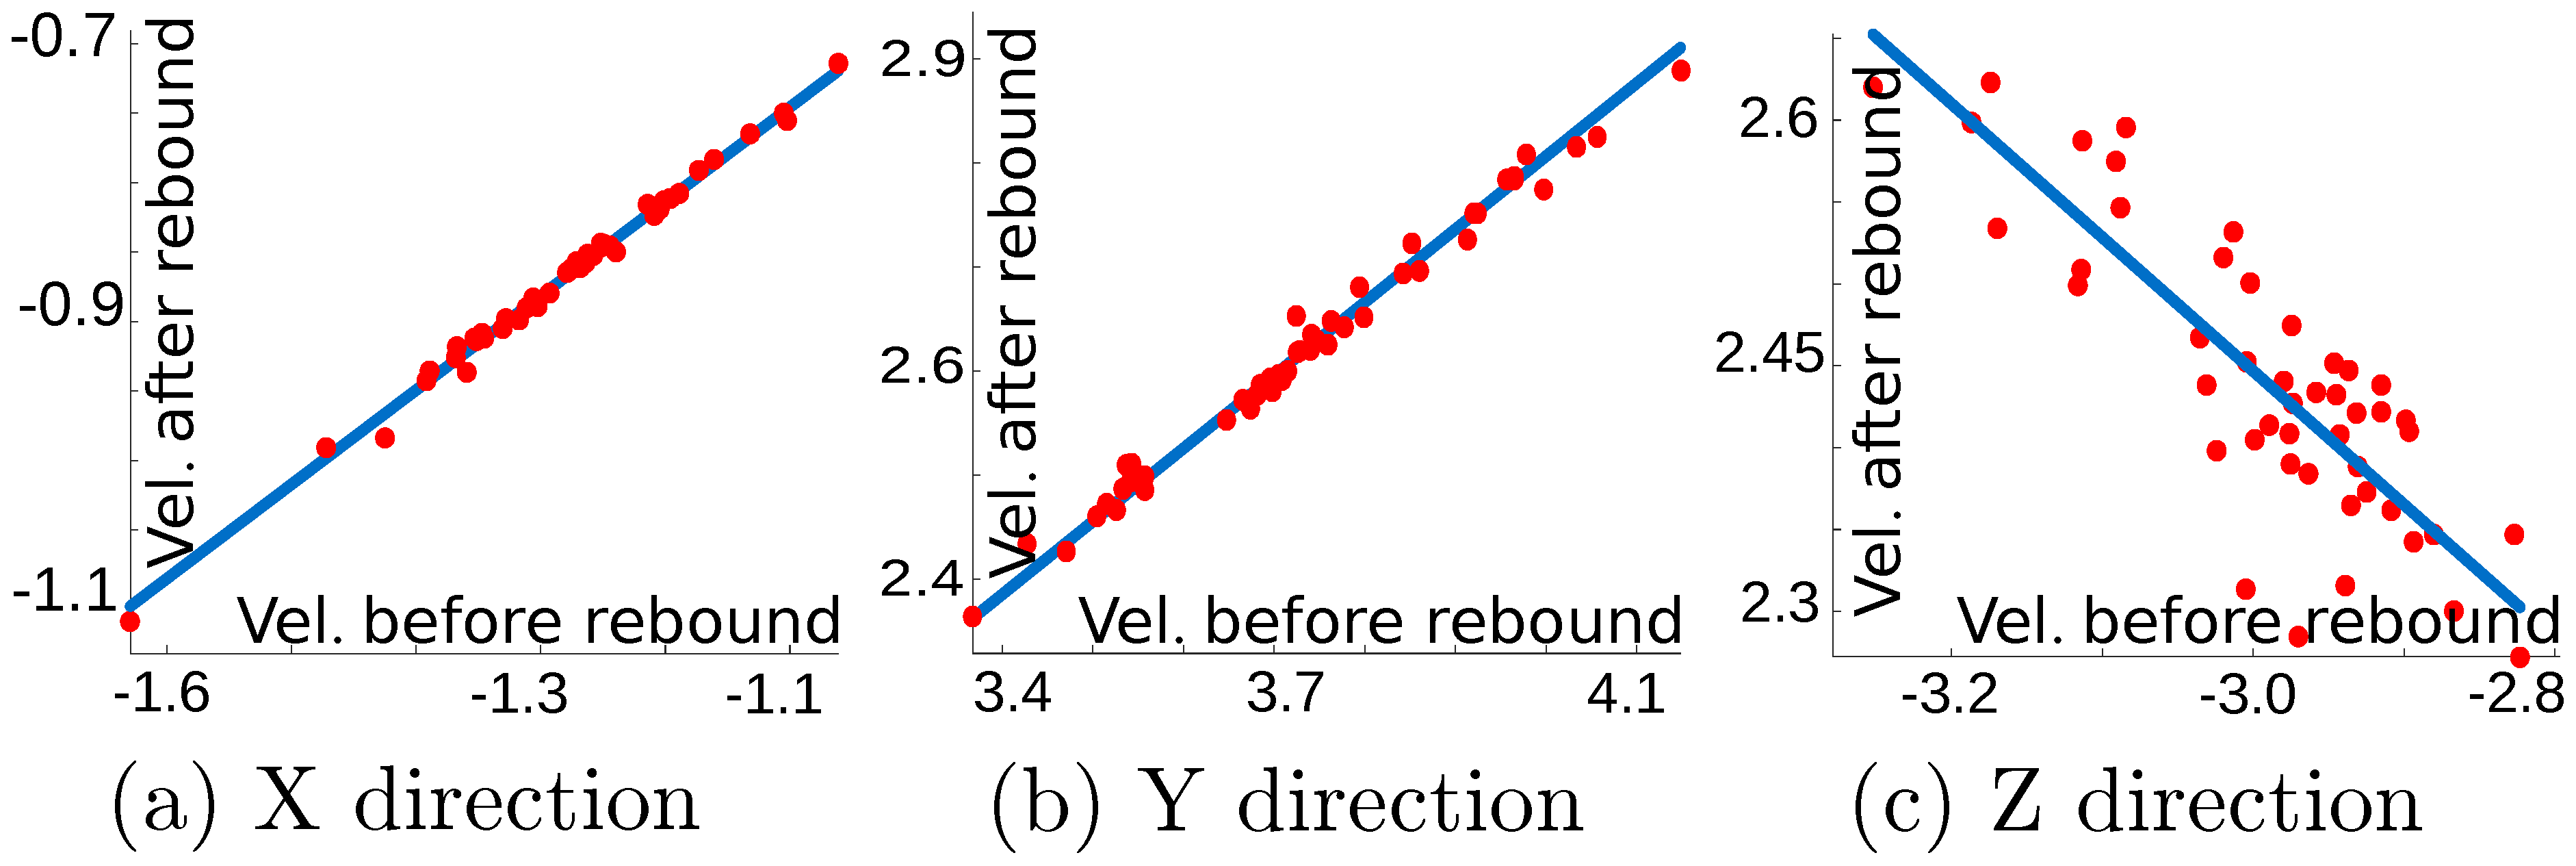
\includegraphics[scale=0.125]{velRebound2.eps}
%	\caption{The plots show the relationship between the velocities before and after rebound. The rebound model parameters are estimated from data with linear regression. It can be seen, especially in the X and Y directions, that the linear model is quite faithful to data. The estimated coefficients are $\epsilon_x = 0.82$, $\epsilon_y = 0.70$ and $\epsilon_z = 0.68$. When the topspin setting is increased in the ballgun to $3000$ rpm, the estimated coefficients increase to $\epsilon_x = 0.96$, $\epsilon_y = 1.18$ and $\epsilon_z = 1.20$.} %The topspin caused by our ball-launcher could be a complicating factor in the vertical direction Z. 
%	\label{fig:rebound}
%\end{figure}
%
In order to estimate the parameters, i.e., $\kappa$ and $\coeffRestitutionRacket$, of the ball-racket interaction model~\eqref{contactModel} we first use the dataset to estimate the striking times $\hitTime_i$. By considering the minimum distance between the ball samples and the demonstrated Cartesian robot trajectories
%
\begin{align}
j_h(i) &= \arg\min_{j} \|\ball_{ij} - \kin_p(\joint_{ij})\|_2, \\
\hitTime_i &\approx t_{ij_h(i)},
\label{strikingTimeEst}
\end{align}
%
\noindent for each trial $i = 1, \ldots N$ we can roughly estimate the striking times $\hitTime_i$. As in estimating the rebound model parameters, the Extended Kalman Smoother is then used to smoothen the ball demonstrations before and after the striking time separately. This procedure results in estimating the incoming and outgoing ball velocities, $\dot{\mathbf{b}}_{\mathrm{in}}(T_i), \, \dot{\ball}_{\mathrm{out}}(T_i)$ as well as the required racket quantities $\racketVel(T_i), \, \normal(T_i)$ at striking times $T_i$. Linear Least Squares is then used with regularizer $\lambda = 0.001$ to estimate the coefficients $\kappa$ and $\coeffRestitutionRacket$. See Table~\ref{tableEstimates} for the estimated values of all the ball model parameters.

An alternative approach would be to estimate all the model parameters together with a smoothing Expectation-Maximization (EM)~\citep{Shumway82} algorithm, yielding additionally covariance estimates for noisy ball observations. 
%
\begin{table}[b!]
	\small\sf %\centering
	%\renewcommand{\arraystretch}{1.3}
	\caption{Ball model parameter estimates}
	\label{tableEstimates}
	\begin{tabular}{c|l|l}
		\toprule
		\bfseries Parameter & \bfseries Description & \bfseries Estimate \\ %	{\small \bfseries Notation}
		\midrule
		$\drag$ & Air drag coefficient & 0.141 \\
		$\lift$ & Lift coefficient & 0.001 \\
		$\gravity$ & Gravity & -9.802 \\
		$\coeffFrictionTable$ & Coeff. of friction of table & 0.102 \\
		$\coeffRestitutionTable$ & Coef. of restitution of table & 0.883 \\
		$\kappa$ & Coeff. of friction of racket & 0.020 \\
		$\coeffRestitutionRacket$ & Coeff. of restitution of racket & 0.788 
		%\bottomrule
	\end{tabular}
\end{table}